\documentclass[12pt]{article}
\usepackage{sbc-template}
\usepackage{graphicx,float,url}
\usepackage[brazil]{babel}   
\usepackage[utf8]{inputenc}  
\usepackage{indentfirst}
\usepackage{listings}

\sloppy
\lstset{numbers=left, numberstyle=\tiny, stepnumber=1, numbersep=5pt,basicstyle=\footnotesize,extendedchars=true,tabsize=2,frame=single, language=lisp}

\title{Similaridade entre textos usando os algoritmos\\ \textit{Dice's Coefficient} e \textit{Longest Common Substring} (LCS)}

\author{Luiz Fellipe Machi Pereira\inst{1}}

\address{
Departamento de Informática -- Universidade Estadual de Maringá (UEM)\\ Maringá -- PR -- Brasil \email{ra103491@uem.br}}

\begin{document} 

\maketitle

\begin{abstract}
Measures of text similarity play an increasingly important role in an era of large, easy flow of information. Such measures can be used for text classification, topic detection, plagiarism detection, among others. In this paper the two algorithms presented, Dice's Coefficient (DC) and Longest Common Substring (LCS), seek the similarity between two texts lexically. The LCS algorithm presented more concise results and tends to present them in a shorter time.
\end{abstract}

\begin{resumo} 
As medidas de similaridade de textos desempenham um papel cada vez mais importante em uma era de grande fluxo facilitado de informações. Tais medidas podem ser usadas para classificação de textos, detecção de tópicos, detecção de plágio, entre outros. Neste artigo os dois algoritmos apresentados, \textit{Dice's Coefficient} (DC) e \textit{Longest Common Substring} (LCS), buscam a semelhança entre dois textos de forma léxica. O algoritmo LCS apresentou resultados mais concisos e tende a apresentá-los em menor tempo.
\end{resumo}

\section{Introdução}

As medidas de similaridade de textos desempenham um papel cada vez mais importante em uma era de grande fluxo facilitado de informações. Tais medidas podem ser usadas para classificação de textos, detecção de tópicos, detecção de plágio, entre outros. Para encontrar similaridade entre textos é fundamental encontrar primeiramente a similaridade entre palavras, para que depois sejam encontradas similaridades entre sentenças, parágrafos e documentos. A semelhança pode ser médica de forma léxica, baseada na cadeia de caracteres usados, ou semântica, baseada no contexto e bases de conhecimento \cite{textsimilarityapproaches}.

Neste artigo os dois algoritmos apresentados, \textit{Dice's Coefficient} (DC) e \textit{Longest Common Substring} (LCS), buscam a semelhança entre dois textos de forma léxica, sendo que o algoritmo DC se pauta na semelhança entre termos e o algoritmo LCS leva em consideração todos os caracteres usados. A análise dos resultados teve como base a implementação de tais algoritmos por meio do paradigma funcional na linguagem Racket.

\newpage

\section{\textit{Longest Common Substring} (LCS)}\label{sec:lcs}

A maior \textit{substring} comum é uma sequência de caracteres que aparece na mesma ordem e de forma contígua em ambas as \textit{strings}. O algoritmo LCS tem como objetivo encontrar o tamanho da maior \textit{substring} comum a duas \textit{strings} \textbf{\textit{S}} e \textbf{\textit{T}}, de tamanhos \textbf{\textit{m}} e \textbf{\textit{n}}, respectivamente \cite{Amir2018LongestCS}. Se usado de Programação Dinâmica (PD), o algoritmo tem complexidade $\mathcal{O}(mn)$ em relação ao tempo \footnote{Complexidade do algoritmo: \url{https://en.wikibooks.org/wiki/Algorithm_Implementation/Strings/Longest_common_substring}}.

\subsection{Implementação do algoritmo em Racket}

A função \textit{lcs-list} abaixo serve como \textit{template} para execução do algoritmo LCS, sendo ela responsável pelo cálculo da maior \textit{substring} comum aos dois textos. A implementação tira vantagem da facilidade de implementação do \textit{memo} para não realizar computações desnecessárias e reduzir o tempo de execução do algoritmo.

\begin{lstlisting}
(define/memoize (lcs-list list1 list2 indice1 indice2)
  (cond 
    [(or (equal? indice1 0) (equal? indice2 0)) 0]
    [(equal? 
      (list-ref list1 (- indice1 1))
      (list-ref list2 (- indice2 1)))
      (+ 1 (lcs-list list1 list2 (- indice1 1) (- indice2 1)))]
    [else
      (max
        (lcs-list list1 list2 indice1 (- indice2 1))
        (lcs-list list1 list2 (- indice1 1) indice2)
      )
    ]
  )
)
\end{lstlisting}

O método lcs faz a normalização do valor recebido da função \textit{lcs-list} para calcular o coeficiente de similaridade entre os textos recebidos.

\begin{lstlisting}
(define (lcs text1 text2)
  (exact->inexact 
    (/ 
      (lcs-list 
        (string->list text1)
        (string->list text2)
        (string-length text1)
        (string-length text2)
      )
      (max (string-length text1) (string-length text2))
    )
  )
)
\end{lstlisting}

\newpage

\section{\textit{Dice's Coefficient} (DC)}\label{sec:dice}

Este método mede a semelhança entre dois conjuntos, não necessariamente entre duas \textit{strings} como o algoritmo de LCS, podendo ser usado para medir o quanto duas sequências de caracteres são semelhantes em relação ao número de bigramas\footnote{Um bigrama ou digrama é uma sequência de dois elementos adjacentes de uma sequência de \textit{tokens}, que normalmente são letras, sílabas ou palavras. Um bigrama é um n-grama para n = 2.} comuns. Este método possui complexidade $\mathcal{O}(n^2)$ em relação ao tempo\footnote{Uma implementação otimizada pode ter sua complexidade em relação ao tempo reduzida para  $\mathcal{O}(n)$: \url{https://en.wikibooks.org/wiki/Algorithm_Implementation/Strings/Dice\%27s_coefficient}}.

Quando tomado como medida para similaridade de um conjunto, o coeficiente para os conjuntos \textbf{\textit{X}} e \textbf{\textit{Y}} pode ser calculado da seguinte maneira:
$$DC = \frac{2 \cdot n_{m}}{(n_{X} + n_{Y})} $$
No qual $n_{m}$ corresponde ao número de bigramas encontrados em ambos os conjuntos, $n_{X}$ o número de bigramas no conjunto \textbf{\textit{X}} e $n_{Y}$ o número de bigramas no conjunto \textbf{\textit{Y}}.

\subsection{Implementação do algoritmo em Racket}

A função \textit{bigrams} abaixo é responsável por criar uma lista com os bigramas de um texto e colocalos em uma lista, tal operação tem complexidade $\mathcal{O}(n)$ em relação ao tempo, onde $n$ é a quantidade de caracteres no texto.

\begin{lstlisting}
(define (bigrams text lista indice)
  (cond
    [(> (+ indice 2) (string-length text)) lista]
    [else 
      (bigrams 
        text
        (append
            lista
            (list (substring text indice (+ indice 2)))
        )
        (add1 indice)
      )
    ]
  )
)
\end{lstlisting}

\newpage

A função \textit{dice-match} abaixo recebe a lista de bigramas dos dois textos e encontra quais estão contidos nas duas listas, retornando a quantidade total de elementos iguais.

\begin{lstlisting}
(define (dice-match list1 list2 i j contador)
  (cond
    [(>= i (length list1)) contador]
    [(>= j (length list2))
        (dice-match list1 list2 (add1 i) 0 contador)
    ]
    [(string=? (list-ref list1 i) (list-ref list2 j)) 
      (dice-match
        list1
        (remove (list-ref list2 j) list2)
        i
        (add1 j)
        (add1 contador)
      )
    ]
    [else (dice-match list1 list2 i (add1 j) contador)]
  )
)
\end{lstlisting}

Por fim o cálculo do coeficiente é realizado, tendo como base o resultado da função \textit{dice-match}. Com o uso da função \textit{exact->inexact} do Racket podemos obter o valor do coeficiente de forma decimal.

\begin{lstlisting}
(define (dice text1 text2)
  (define bigram1 (bigrams text1 (list) 0))
  (define bigram2 (bigrams text2 (list) 0))
  (exact->inexact
    (/ 
      (* 2 (dice-match bigram1 bigram2 0 0 0))
      (+ 
        (length bigram1)
        (length bigram2)
      )
    )
  )
)
\end{lstlisting}

\section{Resultados e discussões}

Nesta seção foram abordadas as metodologias utilizadas e a análise dos resultados obtidos, que indicam um melhor resultado para a técnica LCS.

\subsection{Metodologia utilizada}

Para comparar o desempenho entre os dois algoritmos foram coletados os resultados das execuções de testes com oito diferentes textos de diferentes tamanhos. Para atestar a eficiência dos dois algoritmos implementados, uma comparação foi feita com o resultado produzido pelo site \textit{Countwordsfree} \footnote{Countwordsfree: \url{https://countwordsfree.com/comparetexts}}.

\subsection{Resultados produzidos}

O gráfico presente na Figura~\ref{fig:diferenca} apresenta a execução dos algoritmos para diferentes casos de teste, no qual \textit{text1} e \textit{text2} são textos com quinze palavras aleatórias, \textit{text3} e \textit{text4} textos com vinte e cinza palavras aleatórias, \textit{text5} e \textit{text6} frases com diferentes tamanhos e \textit{text7} \textit{text8} dois algoritmos,escritos na linguagem de programação \textit{C}, com pequenas alterações entre si. O máximo coeficiente ($1.0$) indica a igualdade dos dois textos e o mínimo coeficiente ($0.0$) índice a total diferença entre os textos.

\begin{figure}[H]
    \centering
    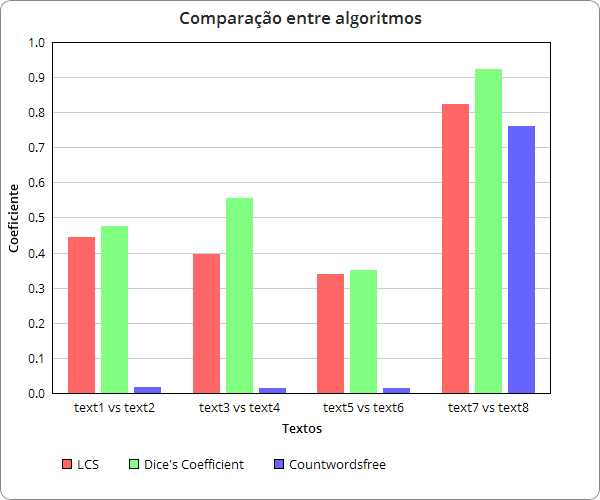
\includegraphics[scale=0.7]{img/diferenca.png}
    \caption{Comparação entre os algoritmos implementados e o disponibilizado pelo site \textit{Countwordsfree}}
    \label{fig:diferenca}
\end{figure}

Em todos os testes apresentados o algoritmo \textit{Dice's Coefficient} apresentou coeficientes maiores de similaridade, o que não necessariamente indica que seja possua desempenho superior ao algoritmo LCS. Tal afirmação dá-se pelo fato de mesmo em textos com palavras aleatórias, primeiro e segundo caso, o coeficiente apresentado é elevado, passando de $0.5$ no segundo caso.

Nota-se também que a maior disparidade de valores ocorre entre o algoritmo \textit{Dice's Coefficient} e os valores dados pelo site \textit{Countwordsfree}. Tais fatores indicam uma maior confiabilidade no método utilizado pelo LCS.

\subsection{Tempo de execução}

Para mensurar o tempo de execução entre os dois métodos apresentados podemos fazer uso da análise de complexidade em relação ao tempo. Como apresentado na Seção~\ref{sec:lcs}, o método LCS apresenta complexidade $\mathcal{O}(mn)$, onde $m$ e $n$ refere-se ao tamanho de cada texto. Ao passo que o método \textit{Dice's Coefficient}, visto na Seção~\ref{sec:dice}, possui complexidade $\mathcal{O}(n^2)$, onde $n$ representa o tamanho do maior texto dentre os inseridos. 

É fácil notar que para textos de mesmo tamanho os dois métodos possuem tempo similar, uma vez que LCS terá a mesma complexidade em relação ao tempo do que o seu concorrente. Porém, para entradas de tamanhos diferentes o algoritmo LCS apresenta vantagem pois tem o número de computações reduzidas.

\section{Conclusão}

Apesar de apresentar maiores coeficientes de similaridade, o método \textit{Dice's Coefficient} aponta menor confiabilidade quando comparado a outros algoritmos, isto é, a diferença em seu resultado se sobressae perante os demais métodos. Além disso o algoritmo LCS apresenta menor complexidade em relação ao tempo, ao mesmo passo que fornece resultados mais próximos aos previamente calculados no site \textit{Countwordsfree}.

\bibliographystyle{sbc}
\bibliography{sbc-template}

\end{document}
